\documentclass[a4paper, 11pt]{article}

\usepackage[utf8x]{inputenc}
\usepackage[english]{babel}
\usepackage{amssymb}
\usepackage{amsmath}
\usepackage[dvips]{graphicx}
\usepackage{floatflt}
\usepackage{psfrag}
\usepackage{subfigure}
\usepackage{booktabs}
%\usepackage{ctable}
\usepackage{siunitx}
\usepackage[a4paper, centering,margin=1.3in, %text={7in,10in},
 bindingoffset=0mm]{geometry}
\usepackage{amsmath}
\usepackage{textcomp}
\usepackage[version=3]{mhchem}
\usepackage{multicol}
\usepackage{hyperref}
\usepackage[nameinlink, capitalize]{cleveref}
%\usepackage{epstopdf}
\usepackage[usenames,dvipsnames]{pstricks}
\usepackage{epsfig}
\usepackage{pst-grad}
\usepackage{pst-plot} % For axes
\usepackage[labelfont=bf, font={small}]{caption}[2004/7/16]
\usepackage{color}

\newcommand{\mate}{\begin{equation}}
\newcommand{\atem}{\end{equation}}
\newcommand{\nona}{\nonumber\\&=&}
\newcommand{\subbo}{\textit}


\title{Photoacoustic observation of the HOWMANYnm absorption line in O$_2$}
\author{Zeno Tornasi, Michele Valentini, Henry Widodo}

\begin{document}
\maketitle\newpage

\tableofcontents\newpage

\section*{Introduction}
\addcontentsline{toc}{section}{Introduction}

In this report we will write about the experiment done during the first and second weeks of August in order to measure one "line"` in the visible part of the absorption spectrum (ATMOSPHERIC BAND/B-BAND?) of the Oxygen molecule using the photoacoustic effect. In order to excite the oxygen molecular orbitals we used a diode laser tuned with an external cavity. INSERT SMALL RESUME OF THE REPORT? FOR EXAMPLE (IN CHAPTER 1 WE WILL TALK ABOUT BLABLA, IN CHAMPTER 2 ABOUT BLIBLI ETC?)

\newpage
\section{Experimental apparatus}
The setup we used featured the typical photoacoustic experiment characteristics. There was a source of light, a laser in our case, impinging on the gas into a cavity. A mechanical chopper provided a modulation of the light in order to match a proper frequency of the cavity. The acoustic signal, detected by microphones, was filtered by a lock-in amplifier referenced with the chopping frequency. The light path was controlled trough optical elements such as mirrors, lenses and beam-splitters. Some standard laboratory instrumentation was used as well, including:
\begin{itemize}
\item generator \item waveform generator \item oscilloscope \item optical fiber spectroscope \item membrane vacuum pump \item etalon \item analogic videocamera \item monitor
\end{itemize}
 We'll now describe in more details the main elements of the apparatus.
\subsection{The laser source}
We used an external cavity laser device, formed by the following elements:
\begin{itemize}
\item a single mode multi-quantum well AlGaInP laser diode\footnote{Hitachi HL6738MG: \url{http://pdf.datasheetcatalog.com/datasheets/50/502031_DS.pdf}}.
 The lasing wavelength could be tuned from about 680 nm to 695 nm by adjusting the driving current and the diode temperature.
\item a temperature controller case\footnote{Thorlabs TCLDM9: \url{http://www.thorlabs.de/Thorcat/1900/TCLDM9-Manual.pdf}} to set the temperature of the diode. 
\item an external cavity, i.e. a setup that feeds back the laser diode with the first diffraction order of a 1800 grooves/mm grating. The external cavity allowed us to better select a given lasing mode, thus getting a smaller emission linewidth. The grating was put on a piezoelectric mechanical actuator, which permitted nm-order adjustments of its position. Since a grating diffracts different frequencies at different angles, moving the grating we could control the frequency fed back to the laser and thus enhanced. This is how we got a fine tuning of the frequency, and how we were able to make the HOWMANYGHz scan to see the absorption line. 
\end{itemize} 
\subsection{The acoustic chamber} 
 The gas to analyze, pure O$_2$ at atmospheric pressure, was contained in a brass chamber, featuring :
\begin{itemize}
\item an internal cavity, about \mbox{13 cm} long, where the gas actually resonated. Other two smaller cavities were present before and after the main cavity. Since we couldn't open the brass chamber, we had no way to accurately measure the dimensions and the position of the main cavity with respect to the other two ones. It should be noticed that our chamber had been recycled from another experiment and was not explicitly thought for the usage we do of it. However, there were two marks on the outer side of the chamber, that were supposed to indicate where the main cavity started and ended.
\item four microphones put about halfway in the chamber, one for each side of it. Due to the fact that the chamber couldn't be opened, we don't know whether the microphones were actually halfway. According to the marks, they were not. In fact, they were 5 mm away from the supposed middle point.
\item an active strain gauge vacuometer\footnote{Edwards ASG-1000-NW16:\vspace{-10pt}
\begin{flushright} \url{http://www.ultimatevacuum.dk/D35725880\%20ASG\%20user\%20manual.pdf}
\end{flushright}} measured the pressure in the chamber. 
\end{itemize}

\newpage
\appendix

\chapter{Extended Cavity Diode Laser (ECDL)}\label{ECDL}
	\section{Introduction to LD tuning}

The light emitted by a diode laser is often practically useless to an experimentalist because of several different reasons:
\begin{itemize}
 \item greatly diverges in an oval shape pattern
 \item because of the small cavity of the laser it has a larger bandwidth which means that diode lasers emit light over a broader range of wavelengths than other kinds of lasers
 \item could have an unstable wavelength due to temperature or current fluctuations.
\end{itemize}

The first problem makes it necessary to collimate the output of the diode laser, that is, bend the diverging light through a lens (or several lenses) so that all the output goes in one direction. One can achieve this result by using a single lens as long as the laser is placed exactly at the focal  point of the lens one chooses. The focal point of a lens is also the point through which all light parallel to its normal axis will converge. Hence, if we place our diode laser at the focal point of our collimating lens all light from the diode laser that passes through the lens will exit parallel to the normal axis and all light that enters the face of the lens at normal incidence will be focused the diode laser.

The broad linewidth of solitary diode laser often reduces their usefulness for spectroscopy applications. To overcome this problem several techniques have been developed, for example:
\begin{itemize}
\item negative electronic feedback
\item resonant optical feedback from a high-finesse optical cavity
\item extended-cavity configurations
\end{itemize}
Among all these techniques that can be used to reduce the laser linewidth down to the kHz range, the extended-cavity configuration with grating feedback has become the most popular. It provides a simple mean to achieve a wide wavelength tuning range and a narrow linewidth.
The external cavity could also solve the instability through optical feedback, severely reducing mode hoping.
In our experiment we used an external cavity in Littrow configuration so we will focus on explaining how such a cavity and it's main components work.
A schematic layout of the extended-cavity laser is outlined in \cref{grating}. The laser system consists of a diode laser as the active medium, a collimating lens and a diffraction grating. The external cavity is formed between the rear facet of the diode laser and the grating as a wavelength selective mirror. The laser frequency depends critically on the optical length of the cavity, which is sensitive to any changes in the refractive index of the cavity media (diode laser, lens, and air) and to changes in the physical cavity length.
The collimation lens of the ECDL (Extended Cavity Diode Laser) is one critical part of attaining optical feedback. The second part of our system that allows optical feedback is the diffraction  grating. 

\begin{figure}[!hbt]\centering
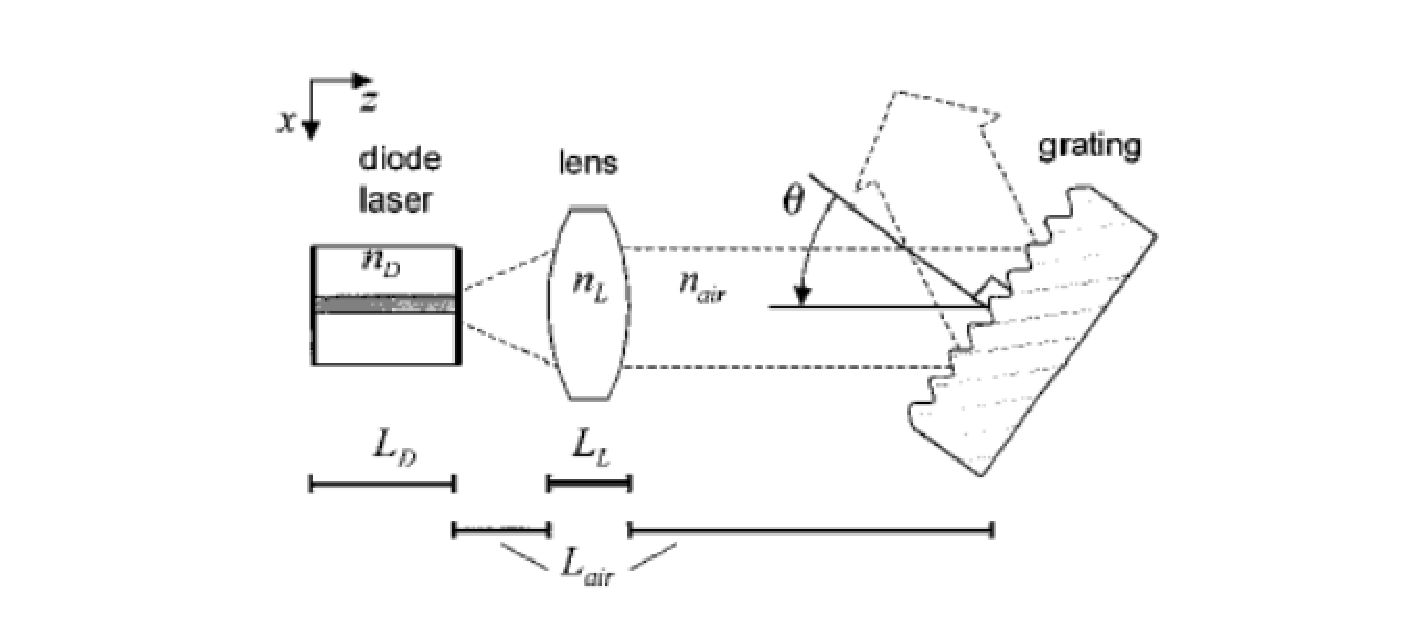
\includegraphics[width=\linewidth, draft=\foto]{eps/littrow1.eps}
\caption{Schematic layout of the extended cavity laser. The total optical path length in the cavity is $L_{\mai{ec}}=L_{\mai{d}}n_{\mai{d}}+L_{\mai{l}}n_{\mai{l}}+L_{\mai{air}}n_{\mai{air}}$}
\label{grating}
\end{figure}

    \section{Diffraction theory for a grating}\label{gratingtheory}
A diffraction grating is a finely scored reflective material that, due to its geometry, allows only certain wavelengths of light incident at an angle to interfere constructively with itself as it is reflected outwards.


 The light diffracted by each groove combines to form a diffracted wavefront. Diffraction by a grating can be visualized from the geometry in \cref{littrow4}, which shows a light ray of wavelength $\lambda$ incident at an angle $\alpha$ and diffracted by a grating along angles $\beta_{\mai{m}}$. These angles are measured from the grating normal, which is the dashed line perpendicular to the grating surface at its center. The sign convention for these angles depends on whether the light is diffracted on the same side or the opposite side of the grating as the incident light. In \cref{littrow3a}, which shows a reflection grating, the angles are  $\alpha>0$ and $\beta_{\mai{1}}>0$ (since they are measured counter-clockwise from the grating normal), while we have $\beta_{\mai{0}}<0$ and $\beta_{\mai{-1}}<0$ (since they are measured clockwise from the grating normal). Diagram \cref{littrow3b} shows the case for a transmission grating.
\begin{figure}[!bht]\centering
\subfigure[A reflection grating: the incident and diffracted rays lie on the same side of the grating.\label{littrow3a}]{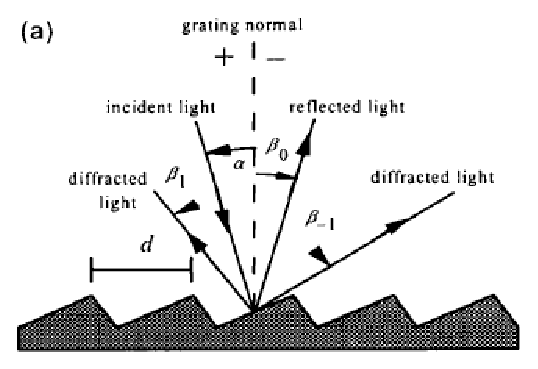
\includegraphics[width=.46\linewidth, draft=\foto]{eps/littrow3a.eps}}
\hfill
\subfigure[A transmission grating: the incident and diffracted rays lies on opposite sides of the grating.\label{littrow3b}]{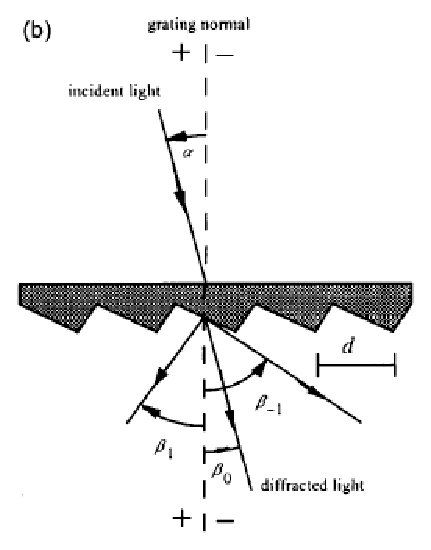
\includegraphics[width=.46\linewidth, draft=\foto]{eps/littrow3b.eps}}
\caption{A comparison between reflection and transmission grating.}
\end{figure}

The formula for constructively diffracted orders of light reflected from a diffraction grating is:(VERIFICO NOMI DEGLI ANGOLI!!!111!!!!111!!!1111)
\mate
d\sin\theta=m\lambda
\label{gianfrancioschio}
\atem
where $d$ is the spacing between reflective surfaces, $\theta$ is the angle of incidence, $\lambda$ is the wavelength of the incident light and $m$ is an integer. One consequence of the above equation is that spectra diffracted off a grating are reproduced at several different angular positions about the grating. The various replications of the spectra are called \textit{orders of diffraction} and obey the following relationship 
\mate
\sin\theta_{\mai{i}} + \sin\theta_{\mai{m}}= N m \lambda
\atem
where $\theta_{\mai{m}}$ is the angle of the $m$th order diffracted beam, $N$ is the spatial frequency of the grating (units mm$^{-1}$), and $\theta_{\mai{i}}$ and $\lambda$ are the incident light angle and wavelength respectively.

When monochromatic light impinges on a grating surface, it is diffracted into discrete directions.
We can easily calculate the  separation between these directions by inverting /ref{gianfrancioschio}.
\mate
\beta[\lambda]=\arcsin\left[\frac{m\lambda}{d} – \sin\alpha\right]
\atem
When $m=0$, the grating acts as a mirror, and the wavelengths are not separated ($\beta=-\alpha$ for all $\lambda$); this is called specular reflection or \textit{the zeroth order}. 
\begin{figure}[!htb]\centering
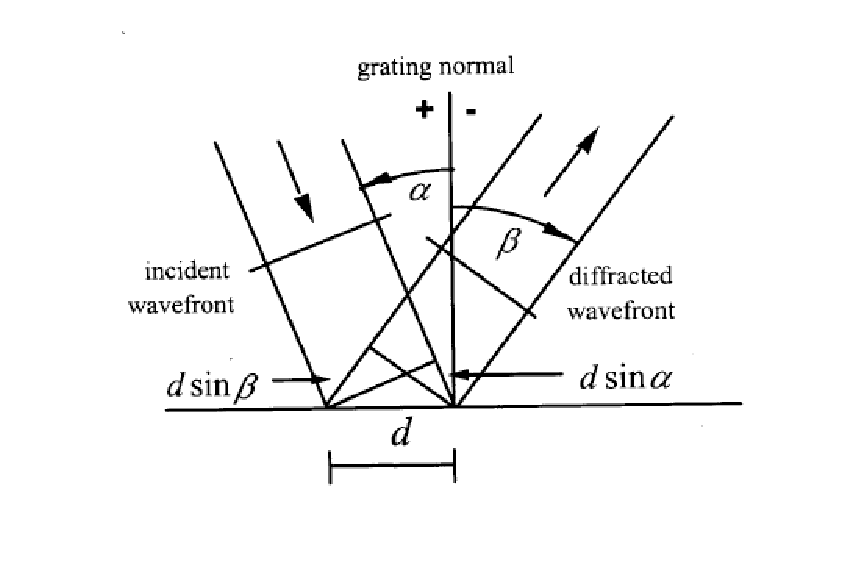
\includegraphics[width=\linewidth, draft=\foto]{eps/littrow4.eps}
\caption{Geometry of diffraction, for planar wavefronts.}
\label{littrow4}
\end{figure}

\section{Littrow configuration ECDL}\label{Littrowsection}
In the Littrow configuration for the external cavity, shown in \cref{littrow2}, the grating is aligned in way such that the first order diffraction from the grating is coupled directly back into the laser, while the zeroth-order diffraction is reflected as the output beam. The lasing wavelength is dependent on the angle of the incident laser beam with respect to the grating, otherwise known as the Littrow angle $\theta$.
There are 3 cavities which set up such configuration:
\begin{enumerate}
\item Laser diode cavity or internal Fabry-P\'{e}rot cavity
\item External cavity between grating and back side of the diode 
\item Parasitic cavity between grating and the front facet of the diode
\end{enumerate}

\begin{figure}[!t]
\centering
%\mbox{
%\begin{minipage}[b]{.60\textwidth}
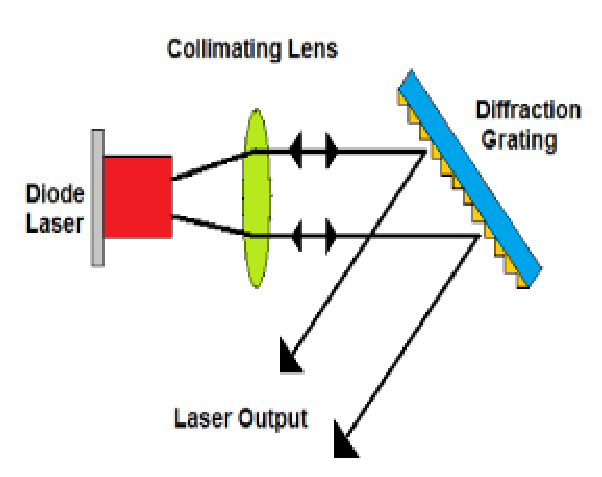
\includegraphics[width=0.7\linewidth, height=5cm, draft=\foto]{eps/littrow2.eps}
%\end{minipage}
%\begin{minipage}[b]{.35\textwidth}
\caption{Schematic diagram of external cavity in Littrow configuration.}
\label{littrow2}
%\end{minipage}}
\end{figure}

The key to the Littrow configuration is the backcoupling of the first-order diffraction beam from the grating into the laser diode. Without this feedback, the Littrow laser cannot achieve single-mode emission and will lase at a wavelength set by the gain peak of the semiconductor active region. When the feedback beam is well aligned, interference fringes are expected in the output beam and the laser remains in single-mode despite small temperature and current changes.

	\section{Main sources of noise in a ECDL}
The frequency of a solitary diode laser is sensitive to variations in the injection current and the junction temperature. This is mainly caused by changes in the refractive index of the active medium and in the optical gain. 
These effects can be reduced in an ECDL but other many noise factors are introduced due to the instability of the optical length of the external cavity.
We will now summarize the main factors which influence the optical length of the cavity.

The optical length of the collimating lens changes with temperature. This is caused by thermal expansion of the material and temperature dependence of the refractive index. Their effects on the laser frequency are described by the relationship 
\mate
\frac{d\nu}{dT_{\mai{l}}}=-\nu\frac{L_{\mai{l}}}{L_{\mai{ec}}}\alpha_{\mai{l}}\left(n_{\mai{l}}-n_{\mai{air}}+\beta_{\mai{l}}n_{\mai{l}}\right)
\label{effect1}
\atem
where $n_{\mai{l}}$ and $n_{\mai{air}}$ are the refractive indices of the lens material and air respectively, and $L_{\mai{l}}$ and $L_{\mai{ec}}$ are the physical length of the lens and the total optical path length of the external cavity, respectively. The thermal expansion coefficient of the lens material is denoted by $\alpha_{\mai{l}}$ and the relative temperature coefficient of the refractive index by $\beta_{\mai{l}}$. 

The refractive index of air is mainly sensitive to variations in pressure $p$ and temperature $T_{\mai{air}}$.The variations in the laser frequency due to these changes are described by
\begin{align}
\frac{d\nu}{dp}=-\nu\frac{L_{\mai{air}}}{L_{\mai{ec}}}\frac{dn_{\mai{air}}}{dp}\label{effect2}\\
\frac{d\nu}{dT_{\mai{air}}}=-\nu\frac{L_{\mai{air}}}{L_{\mai{ec}}}\frac{dn_{\mai{air}}}{dT_{\mai{air}}}
\label{effect3}
\end{align}
where $L_{\mai{air}}$ is the cavity length containing air.	

The mechanical structure of the cavity often contains micrometric screws and piezoelectric transducers (PZTs) for wavelength control. The sensitivity of the laser frequency to thermal expansion of these parts can be written as
\mate
\frac{d\nu}{dT_{\mai{m}}}=\pm\nu\frac{L_{\mai{m}}}{L_{\mai{ec}}}\alpha_{\mai{m}}
\label{effect4}
\atem
where $L_{\mai{m}}$ and $\alpha_{\mai{m}}$ are the length and the thermal expansion coefficient of the mechanical part, respectively.

A transverse displacement along $x$ axis of the collimating lens with respect to the laser diode changes the beam direction. This causes a frequency shift due to a change in the cavity length. For a small displacement, the frequency shift can be written as
\begin{align}
\frac{d\nu}{dx}=\frac{\nu\tan\theta}{f_{\mai{l}}}
\label{displacement}\\
\frac{d\nu_{\mai{g}}}{dT}=-\nu_{\mai{g}}\alpha_{\mai{g}}
\label{displacement2}
\end{align}
where $f_{\mai{l}}$ is the focal length of the lens and $\theta$ is the angle between the grating normal and the incident beam, while $\nu_{\mai{g}}$ and $\alpha_{\mai{g}}$ are the central frequency of the grating feedback and the grating thermal expansion coefficient respectively. The displacement of the lens can be caused, for example, by asymmetric thermal expansion relative to the optical axis or by mechanical vibration of the lens holder. 

There are additional effects that influence mainly the short-term frequency stability of the laser: current- and PZT driver noise, mechanical vibrations, acoustic disturbances, and rapid changes in the refractive index of air caused by air flow. All of these factors have an effect on the length of the external cavity and, consequently, generate frequency modulation of the laser.

\newpage\section{The etalon}
\subsection{Introduction}
The etalon is an optical device made of two perfectly parallel semi-reflecting surfaces. It can be thought as a Fabry-P\'erot cavity which walls are fixed. This geometry can be implemented either with an air-based or a solid design. The first one consist in two surfaces separated by air, one of which usually can be moved via piezoelectric actuators. The second one is just made from a piece of glass (or other materials suitable for the desired application) with a partially reflecting coating covered facets (\cref{solidstate}). While the air based etalons make longer cavities, thus more precise, they are extremely delicate and cumbersome to manage, mostly because the two surfaces must be kept parallel within hundredths of wavelength. The solid state ones, on the other hand, are usually smaller and less performing, but way more robust and easier to use.

Every time the impinging beam encounters one of the two optical surfaces the light is partially reflected and partially transmitted. Multiple reflections occur inside the two surfaces leading to an infinite number of rays departing from the interferometer in both the transmitted and reflected directions. Contiguous beams differ for a constant phase and this causes an interference pattern, as shown in \cref{etalonmonitor}.

\begin{figure}[!h]\centering
\begin{minipage}[t]{0.46\textwidth}\centering
\includegraphics[width=\linewidth, height=5cm]{eps/etalon5.eps}
\caption{Solid state etalons.}
\label{solidstate}
\end{minipage}
\hfill
\begin{minipage}[t]{0.46\textwidth}\centering
\includegraphics[width=\linewidth, height=5cm]{eps/thering.eps}
\caption{The etalon diffraction pattern seen through our videocamera.}
\label{etalonmonitor}
\end{minipage}
\end{figure}

\subsection{Theoretical treatment}
To derive the phase difference between two adjacent beams, let's begin calculating the difference in their optical paths (\cref{fig:angoli}). We thus choose two parallel beams, such as $OB$ and $CD$, and draw a wavefront perpendicular to them, $AC$. 
\begin{figure}[!h]
\centering
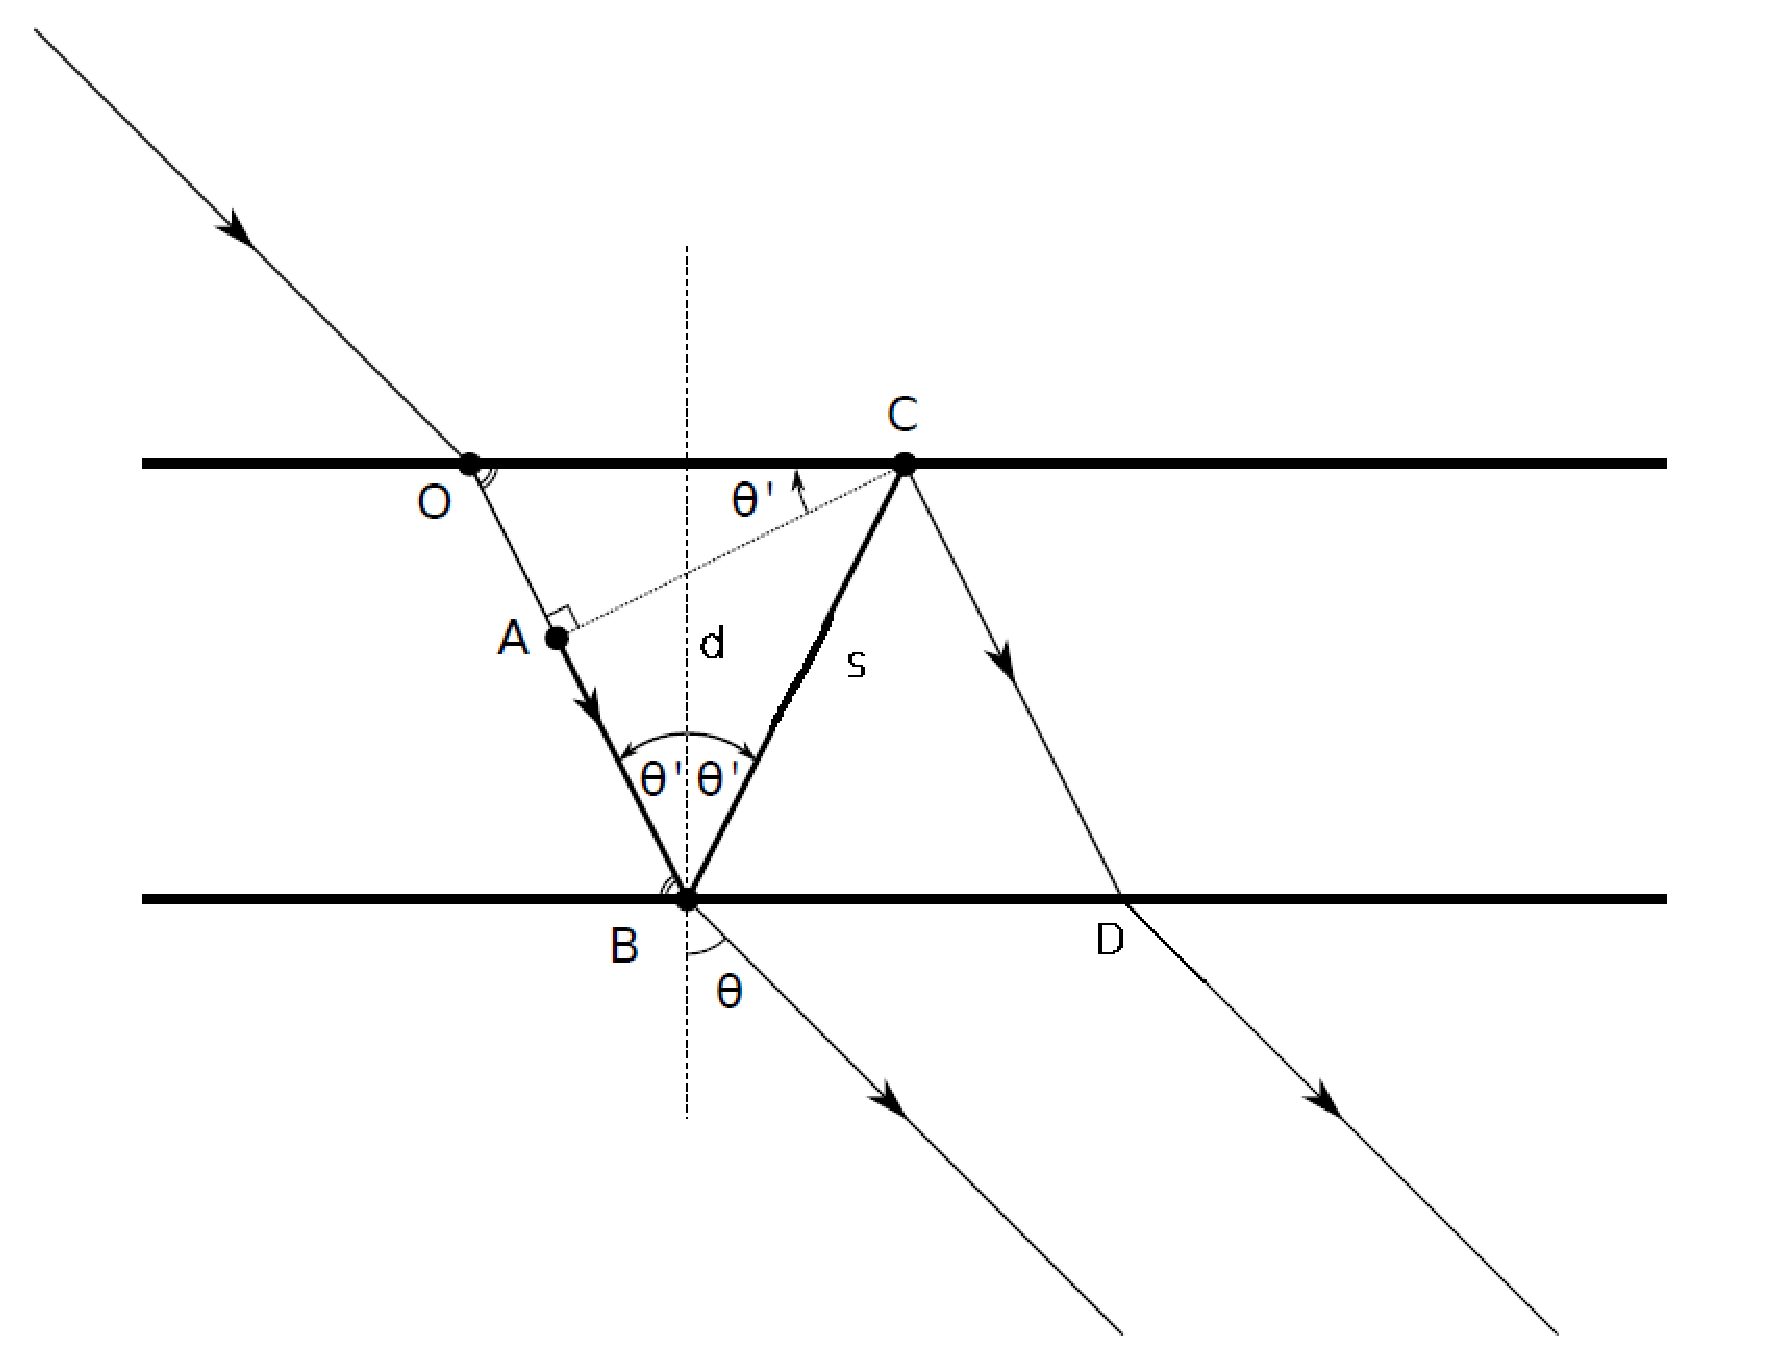
\includegraphics[width=.8\linewidth]{eps/angoli.eps}
\caption{The impinging beam changes direction due to refraction index difference between the air and the glass, the angles $\theta$ and $\theta'$ being related to the refraction indices $n$ and $n'$ by Snell's law.}
\label{fig:angoli}
\end{figure}
The optical path difference between $A$ and $C$ is given by
\begin{equation}
\overline{ABC}=\overline{AB}+\overline{BC}
\end{equation}
 We call $d$ the width of the etalon, and $s$ the distance traveled by the beam from one surface to the other one, so that
\begin{equation}
\overline{BC}=\overline{OB}\equiv s=\frac{d}{\cos\theta'}.
\end{equation} 
From elementary geometry considerations we get the following relationships:
\begin{eqnarray}
\overline{AB}&=&\overline{OB}-\overline{OA}\\
\overline{OA}&=&\sqrt{\overline{OC}^2-\overline{AC}^2}\\
\overline{OC}&=&2s\sin\theta'\\
\overline{AC}&=&s\sin(2\theta')
\end{eqnarray}
Then we write
\begin{eqnarray}
\nonumber\overline{OA}&=&\sqrt{4s^2\sin^2\theta'-s^2\sin^2(2\theta')}\\
\nonumber&=&\sqrt{4s^2\sin^2\theta'\left(1-\frac{\sin^2(2\theta')}{4\sin^2\theta'}\right)}\\
\nonumber&=&2s\sin\theta'\sqrt{1-\cos^2\theta'}\\
&=&2s\sin^2\theta'
\end{eqnarray}
Putting all together we get the optical path difference

\begin{eqnarray}
\nonumber\overline{ABC}&=&\overline{AB}+\overline{BC}\\
\nonumber&=&\overline{OB}-\overline{OA}+\overline{BC}\\
\nonumber&=&s-2s\sin^2\theta'+s\\
\nonumber&=&2s(1-\sin^2\theta')\\
\nonumber&=&2s\cos^2\theta'\\
&=&2d\cos\theta'.
\end{eqnarray}

If the incident light has wavelength $\lambda_0$ in the vacuum and the etalon medium has refractive index $n'$, the light wave vector inside the medium is
 \begin{equation}
k=\frac{2\pi}{\lambda_0}n'
\end{equation}
and the phase shift between two adjacent rays is 
\mate
\Delta=k\cdot\overline{ABC}=\frac{4\pi}{\lambda_0}n'd\cos\theta'
\label{phase}
\atem

Now, indicating by $T$ the overall etalon transmission coefficient and by $R$ the reflection coefficient correspondig to one round-trip, the total amplitude of the electric field in some point after the etalon is the sum of those of the subsequent rays
\mate
E_T=E_0T+E_0TRe^{i\Delta}+E_0TR^2e^{i2\Delta}+E_0TR^3e^{i3\Delta}+\dots
\atem
which is nothing but the geometrical series, that can be summed up ($|Re^{i\Delta}|<1$) to yield 
\mate
E_T=E_0T\sum_{j}\left(Re^{i\Delta}\right)^j=\frac{E_0T}{1-Re^{i\Delta}}
\atem

What we observe is actually the transmitted intensity 

\mate
I_T=|E_T|^2=|E_0|^2\frac{T^2}{|1-Re^{i\Delta}|^2}
\atem

The denominator can be rewritten as
\begin{eqnarray}
|1-Re^{i\Delta}|&=&(1-Re^{i\Delta})(1-Re^{-i\Delta})
\nona 1-R(e^{i\Delta}+e^{-i\Delta})+R^2
\nona 1-2R\cos\Delta+R^2
\nona 1-2R\left(1-2\sin^2\frac{\Delta}{2}\right)+R^2
\nona 1-2R+4R\sin^2\frac{\Delta}{2}+R^2
\nona\nonumber (1-R)^2+4R\sin^2\frac{\Delta}{2}\\
&=& (1-R)^2\left(1+\frac{4R}{(1-R)^2}\sin^2\frac{\Delta}{2}\right)
\end{eqnarray}

So that the transmitted intensity becomes
\mate
I_T=I_0\frac{T^2}{(1-R)^2}\frac{1}{\left(1+\frac{4R}{(1-R)^2}\sin^2\frac{\Delta}{2}\right)}
\label{intensity}
\atem

One defines a \textit{peak constant}
\mate
C_{\mbox{peak}}\equiv\frac{T^2}{(1-R)^2}
\atem

which is equal to 1 for an ideal surface such that $1=R+T$. In a real surface, instead, some absorption $A$ is present, so that $1=R+T+A$. The peak constant in this case can be rewritten as
\mate
C_{\mbox{peak}}=\frac{(1-A-R)^2}{(1-R)^2}=\left(1-\frac{A}{1-R}\right)^2
\atem 

Furthermore we shall define the \textit{coefficient of finesse}\footnote{Not to be confused with the \textit{finesse} defined further in this discussion at pg.\ \pageref{finesse}. These two parameters are strongly correlated, though, and literature is not uniform on which of the two is to be called "finesse".}
\mate
F\equiv\frac{4R}{(1-R)^2}.
\atem

In the ideal etalon case we have $A\simeq0$, which implies $C_{\mbox{peak}}\simeq1$,  so that \cref{intensity} eventually reduces to
\mate
I_T=I_0\ \frac{1}{1+F\sin^2\frac{\Delta}{2}}
\atem

The transmitted intensity is thus given by the constant input intensity value, modulated by the so called \textit{Airy function} plotted in \cref{Airyplot}
\mate
\frac{I_T}{I_0}=\frac{1}{1+F\sin^2\frac{\Delta}{2}}\equiv A[F;\Delta]
\atem

\begin{figure}[htb]\centering
% GNUPLOT: LaTeX picture with Postscript
\begingroup
  \makeatletter
  \providecommand\color[2][]{%
    \GenericError{(gnuplot) \space\space\space\@spaces}{%
      Package color not loaded in conjunction with
      terminal option `colourtext'%
    }{See the gnuplot documentation for explanation.%
    }{Either use 'blacktext' in gnuplot or load the package
      color.sty in LaTeX.}%
    \renewcommand\color[2][]{}%
  }%
  \providecommand\includegraphics[2][]{%
    \GenericError{(gnuplot) \space\space\space\@spaces}{%
      Package graphicx or graphics not loaded%
    }{See the gnuplot documentation for explanation.%
    }{The gnuplot epslatex terminal needs graphicx.sty or graphics.sty.}%
    \renewcommand\includegraphics[2][]{}%
  }%
  \providecommand\rotatebox[2]{#2}%
  \@ifundefined{ifGPcolor}{%
    \newif\ifGPcolor
    \GPcolorfalse
  }{}%
  \@ifundefined{ifGPblacktext}{%
    \newif\ifGPblacktext
    \GPblacktexttrue
  }{}%
  % define a \g@addto@macro without @ in the name:
  \let\gplgaddtomacro\g@addto@macro
  % define empty templates for all commands taking text:
  \gdef\gplbacktext{}%
  \gdef\gplfronttext{}%
  \makeatother
  \ifGPblacktext
    % no textcolor at all
    \def\colorrgb#1{}%
    \def\colorgray#1{}%
  \else
    % gray or color?
    \ifGPcolor
      \def\colorrgb#1{\color[rgb]{#1}}%
      \def\colorgray#1{\color[gray]{#1}}%
      \expandafter\def\csname LTw\endcsname{\color{white}}%
      \expandafter\def\csname LTb\endcsname{\color{black}}%
      \expandafter\def\csname LTa\endcsname{\color{black}}%
      \expandafter\def\csname LT0\endcsname{\color[rgb]{1,0,0}}%
      \expandafter\def\csname LT1\endcsname{\color[rgb]{0,1,0}}%
      \expandafter\def\csname LT2\endcsname{\color[rgb]{0,0,1}}%
      \expandafter\def\csname LT3\endcsname{\color[rgb]{1,0,1}}%
      \expandafter\def\csname LT4\endcsname{\color[rgb]{0,1,1}}%
      \expandafter\def\csname LT5\endcsname{\color[rgb]{1,1,0}}%
      \expandafter\def\csname LT6\endcsname{\color[rgb]{0,0,0}}%
      \expandafter\def\csname LT7\endcsname{\color[rgb]{1,0.3,0}}%
      \expandafter\def\csname LT8\endcsname{\color[rgb]{0.5,0.5,0.5}}%
    \else
      % gray
      \def\colorrgb#1{\color{black}}%
      \def\colorgray#1{\color[gray]{#1}}%
      \expandafter\def\csname LTw\endcsname{\color{white}}%
      \expandafter\def\csname LTb\endcsname{\color{black}}%
      \expandafter\def\csname LTa\endcsname{\color{black}}%
      \expandafter\def\csname LT0\endcsname{\color{black}}%
      \expandafter\def\csname LT1\endcsname{\color{black}}%
      \expandafter\def\csname LT2\endcsname{\color{black}}%
      \expandafter\def\csname LT3\endcsname{\color{black}}%
      \expandafter\def\csname LT4\endcsname{\color{black}}%
      \expandafter\def\csname LT5\endcsname{\color{black}}%
      \expandafter\def\csname LT6\endcsname{\color{black}}%
      \expandafter\def\csname LT7\endcsname{\color{black}}%
      \expandafter\def\csname LT8\endcsname{\color{black}}%
    \fi
  \fi
  \setlength{\unitlength}{0.0500bp}%
  \begin{picture}(7200.00,5040.00)%
    \gplgaddtomacro\gplbacktext{%
      \csname LTb\endcsname%
      \put(946,704){\makebox(0,0)[r]{\strut{} 0}}%
      \csname LTb\endcsname%
      \put(946,1439){\makebox(0,0)[r]{\strut{} 0.2}}%
      \csname LTb\endcsname%
      \put(946,2174){\makebox(0,0)[r]{\strut{} 0.4}}%
      \csname LTb\endcsname%
      \put(946,2909){\makebox(0,0)[r]{\strut{} 0.6}}%
      \csname LTb\endcsname%
      \put(946,3644){\makebox(0,0)[r]{\strut{} 0.8}}%
      \csname LTb\endcsname%
      \put(946,4379){\makebox(0,0)[r]{\strut{} 1}}%
      \csname LTb\endcsname%
      \put(1078,484){\makebox(0,0){\strut{}$-3\pi$}}%
      \csname LTb\endcsname%
      \put(2032,484){\makebox(0,0){\strut{}$-2\pi$}}%
      \csname LTb\endcsname%
      \put(2986,484){\makebox(0,0){\strut{}$-\pi$}}%
      \csname LTb\endcsname%
      \put(3941,484){\makebox(0,0){\strut{}$0$}}%
      \csname LTb\endcsname%
      \put(4895,484){\makebox(0,0){\strut{}$\pi$}}%
      \csname LTb\endcsname%
      \put(5849,484){\makebox(0,0){\strut{}$2\pi$}}%
      \csname LTb\endcsname%
      \put(6803,484){\makebox(0,0){\strut{}$3\pi$}}%
      \put(176,2541){\rotatebox{-270}{\makebox(0,0){\strut{}$A[F;\Delta]$}}}%
      \put(3940,154){\makebox(0,0){\strut{}Phase shift ($\Delta$)}}%
      \put(3940,4709){\makebox(0,0){\strut{}The Airy function for different values of F}}%
    }%
    \gplgaddtomacro\gplfronttext{%
      \csname LTb\endcsname%
      \put(4336,4232){\makebox(0,0)[l]{\strut{}F = 1}}%
      \csname LTb\endcsname%
      \put(4336,4012){\makebox(0,0)[l]{\strut{}F = 10}}%
      \csname LTb\endcsname%
      \put(4336,3792){\makebox(0,0)[l]{\strut{}F = 100}}%
    }%
    \gplbacktext
    \put(0,0){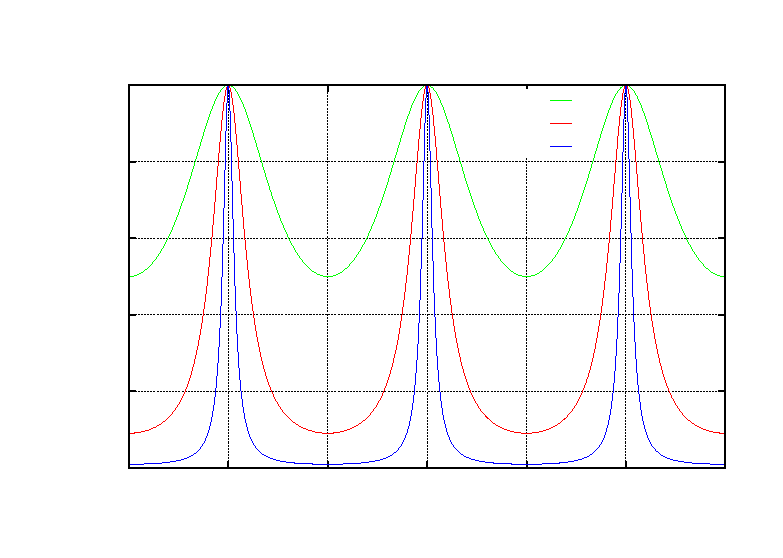
\includegraphics{eps/Airy}}%
    \gplfronttext
  \end{picture}%
\endgroup

\caption{The Airy function peaks when the phase shift is an integer multiple of $2\pi$. As the finesse coefficient increases, the peaks become more sharp and their position is better defined.}
\label{Airyplot}
\end{figure}
\subsection{Interference pattern}
As is clear from \cref{Airyplot}, the interference maxima take place for $\Delta=2m\pi$, where $m$ is an integer representing the order of diffraction.
From \cref{phase} we have
\mate
m=\frac{2n'}{\lambda_0}d\cos\theta'
\label{ordine}
\atem
Looking at \cref{intensity} we define the intensity at the maximum and at the minimum as
\begin{eqnarray}
I_{\mbox{max}}&=&\frac{I_T[\Delta=2m\pi]}{I_{0}}=C_{\mbox{peak}}=\frac{T^2}{(1-R)^2}\\
I_{\mbox{min}}&=&\frac{I_T[\Delta=(2m+1)\pi]}{I_{0}}=\frac{T^2}{(1-R)^2+4R}=\frac{T^2}{(1+R)^2}
\end{eqnarray}
We shall now define a \textit{contrast factor}
\mate
\mathcal{C}\equiv\frac{I_{\mbox{max}}}{I_{\mbox{min}}}=\left(\frac{1+R}{1-R}\right)^2=1+F
\atem
which is also a useful parameter in the characterization of an etalon.

To describe how defined are the peaks, we have to consider their full width at half maximum (FWHM). Thus we observe the points around a maximum whose intensity is $I_{T}=I_{\mbox{max}}/2$. They have a phase shift 
\mate
\Delta=2m\pi\pm\frac{\varepsilon}{2}
\atem

where $\varepsilon$ is now the FWHM expressed as a phase. Putting this into \cref{intensity} we get the identity

$$\frac{1}{2}=\frac{1}{1+F\sin^2\frac{\varepsilon}{4}}\quad;$$ $$F\sin^2\frac{\varepsilon}{4}=1$$

If now we approximate $\sin\frac{\varepsilon}{4}\simeq\frac{\varepsilon}{4}$ we get the phase expression for the FWHM, as a function of the coefficient of finesse $F$
\mate
\varepsilon=\frac{4}{\sqrt{F}}
\atem
Since two contiguous maxima are separated by a phase of $2\pi$, we can do the ratio between the peaks separation and their width, getting a very important parameter which is called the \textit{finesse} of the etalon
\mate
\mathcal{F}\equiv\frac{2\pi}{\varepsilon}=\frac{\pi}{2}\sqrt{F}=\frac{\pi\sqrt{R}}{1-R}
\label{finesse}
\atem
\subsection{Etalon as a spectroscope}
It is possible to build a direct relationship between the angular separation of the rings and the wavelength $\lambda_0$ of the incident light.
We put ourself under the approximation of nearly perpendicular incident light, so that
$$\sin\theta'\simeq\theta'$$$$\sin\theta\simeq\theta$$
Snell's law then simplifies to
$$\frac{\sin\theta'}{n'}=\frac{\sin\theta}{n}\quad\Rightarrow\quad\frac{\theta'}{n'}=\frac{\theta}{n}$$
The small angles approximation also implies
\begin{eqnarray} 
\nonumber\cos\theta'&\simeq&1-\frac{\theta'^2}{2}\\&\simeq&1-\left(\frac{n'}{n}\right)^2\frac{\theta^2}{2}\nonumber
\end{eqnarray}
These approximations being valid, we recall \cref{ordine}
$$m=\frac{2n'}{\lambda_0}d\cos\theta'\quad\Rightarrow\quad m=\frac{2n'}{\lambda_0}d\left(1-\left(\frac{n'}{n}\right)^2\frac{\theta^2}{2}\right)$$
Inverting this one we find
NON SI CAPISCE DA DOVE LA TIRA FUORI E COME, CI SONO CONTI OSCURI [$\dots$]
The angle for the p\textit{th} order is
\mate
\theta_p=\frac{1}{n}\sqrt{\frac{n'\lambda_0}{d}}\sqrt{p-1+e}
\atem
and if we focus the rings onto a screen with a convergent lens, of focal ratio $f$, the diameter of the bright ring is
\mate
D^2_p=(2f\theta_p)^2=\frac{4n'\lambda_0f^2}{n^2d}(p-1+e)
\atem

\end{document}